\documentclass[20pt]{article}

\usepackage[english]{babel}
\usepackage[utf8x]{inputenc}
% \usepackage{amsmath}
\usepackage{graphicx}
\usepackage[margin=0.8in]{geometry}

\title{AS205:Ocean Dynamics(Assignment 3)}
\author{Parag Shende}

\begin{document}
\maketitle
\hrule

\section*{Introduction}

We describe the seasonal mixed layer depth of North Indian Ocean using two criterias: Temperature and Density. The difference of the two
mixed layer calculated by both the criterias gives us the barrier layer thickness.

\section*{Datasets}

The datasets used in this analysis is as follows:

\begin{itemize}
    \item \textbf{Potential temperature} : WOA18(World Ocean Atlas) data.
    \item \textbf{Density} : WOA18(World Ocean Atlas) data.
\end{itemize}

\section*{Methodology}

The datasets are choosen for the domain of $40^{\circ} E$ to $100^{\circ}E$ and $0^{\circ} N$ to $25^{\circ} N$. This covers the
North Indian ocean. We then calculate the seasonal mean with the following seasons:

\begin{itemize}
    \item \textbf{Summer Monsoon} : June, July, August, September(JJAS)
    \item \textbf{Winter Monsoon} : November, December, January, February(NDJF)
\end{itemize}


The temperature criteria gives us a mixed layer depth called isothermal layer depth(ILD). This is determined as the depth at which the 
temperature difference from the 10m depth is greater than $0.2^{\circ}$.


The density criteria gives us a depth that is such that the density is $0.125 kg/m^{3}$ more than that at 10m depth.

The difference in the mixed layer calculated by above two criterias gives us the barrier layer thickness.

\section*{Summer}

\begin{figure}
    \centering
    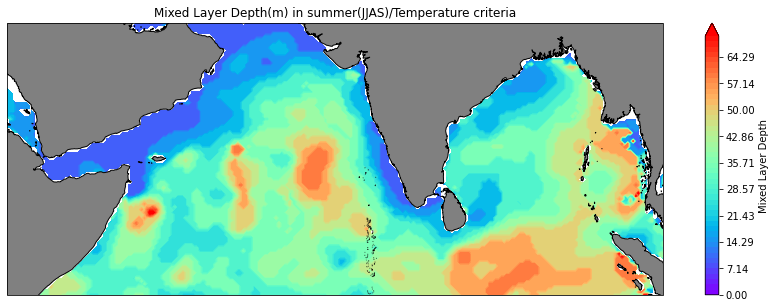
\includegraphics[width=0.88\textwidth]{temp_summer.png}
    \caption{Mixed layer depth(temperature criteria) in summer in $m$}
\end{figure}

\begin{figure}
    \centering
    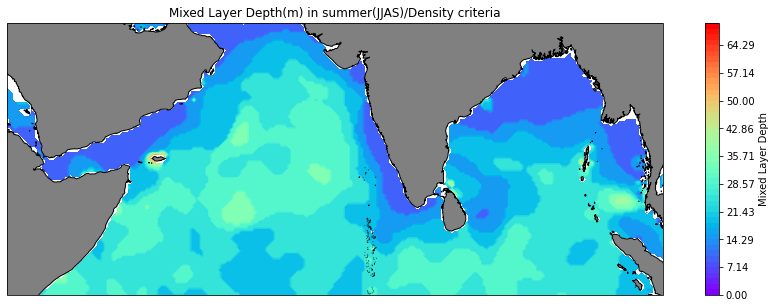
\includegraphics[width=0.88\textwidth]{density_summer.png}
    \caption{Mixed layer depth(density criteria) in summer in $m$}
\end{figure}

\begin{figure}
    \centering
    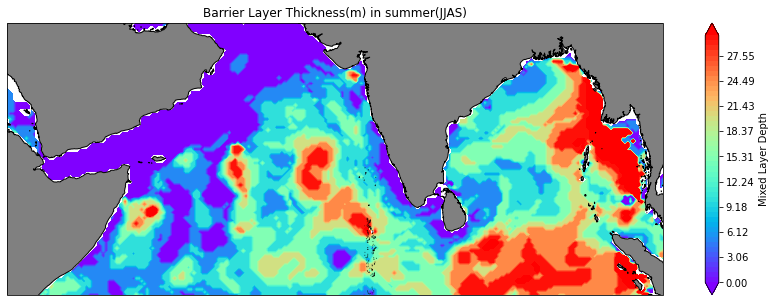
\includegraphics[width=0.88\textwidth]{blt_summer.png}
    \caption{Barrier layer thickness in summer in $m$}
\end{figure}

\begin{itemize}
    \item The seasonal mean mixed layer calculated for summer by both criterias is shown in Figure 1,2.
    \item We see that the mixed layer depth given by both criterias is greater in Arabian Sea than Bay of Bengal.
    \item The barrier layer thickness is greater in Bay of Bengal than the Arabian sea in line with observations.
\end{itemize}

\section*{Winter}

\begin{figure}
    \centering
    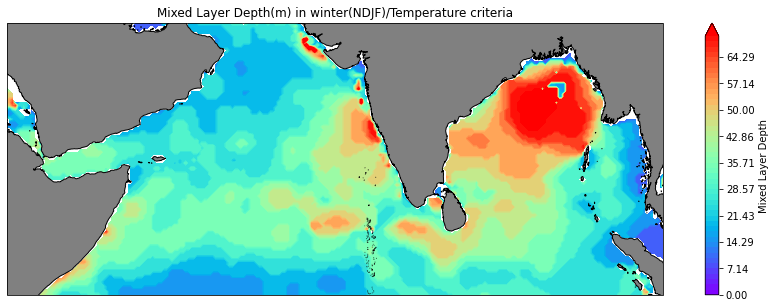
\includegraphics[width=0.88\textwidth]{temp_winter.png}
    \caption{Mixed layer depth(temperature criteria) in winter in $m$}
\end{figure}

\begin{figure}
    \centering
    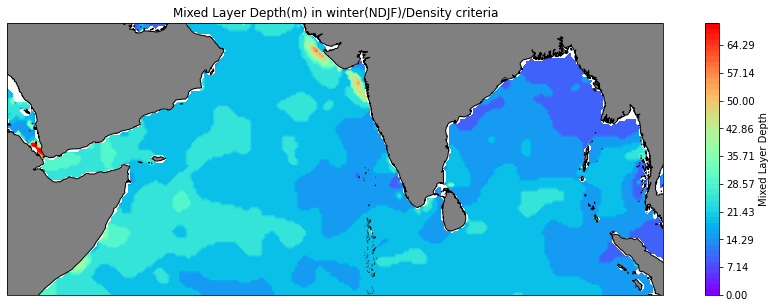
\includegraphics[width=0.88\textwidth]{density_winter.png}
    \caption{Mixed layer depth(density criteria) in winter in $m$}
\end{figure}

\begin{figure}
    \centering
    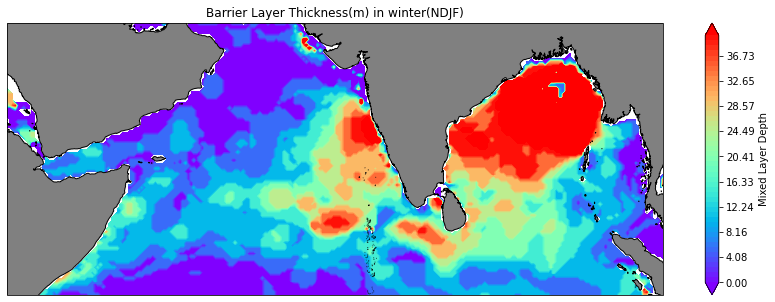
\includegraphics[width=0.88\textwidth]{blt_winter.png}
    \caption{Barrier layer thickness in winter in $m$}
\end{figure}

\begin{itemize}
    \item The seasonal mean mixed layer calculated for winter by both criterias is shown in Figure 4,5.
    \item We see that the mixed layer depth given by density criteria is greater in Arabian Sea as compared to Bay of Bengal.
    \item The temperature criteria gives a deeper isothermal layer in Bay of Bengal.
    \item The barrier layer thickness is greater in Bay of Bengal as compared to Arabian Sea.
\end{itemize}

\section*{Conclusions}

\begin{itemize}
    \item We compared the seasonal means of mixed layer depth of North Indian Ocean by two different criterias.
    \item The calculations match the observations.
\end{itemize}

\end{document}